\documentclass[12pt,oneside]{book}
\pagestyle{headings}

% Note that the line below could be modified to suit a
% particular system since the "geometry" package behaves
% differently in Unix, Windows and Mac, especially for the
% top margins.
% Adjust the parameter "top" (measuring the height of the
% space allocated to a header) and "headsep" (measuring
% the distance from the bottom of the header to the
% first line of text.
\usepackage[top=1.3in,left=1.5in,bottom=1in,right=1in,headsep=0.5in]{geometry}

\usepackage{setspace}
\onehalfspacing
%\doublespacing

% Headers and footers for thesis
\usepackage{fancyhdr}

\markboth{}{}
\newcommand\startchapter[1]{\chapter{#1}\thispagestyle{myheadings}}
\newcommand\startappendix[1]{\chapter{#1}\thispagestyle{myheadings}}
\newcommand\startfirstchapter[1]{\chapter{#1}}

% Manual addition of section to Table of Contents
\newcommand\TOCadd[1]{\newpage\phantomsection\addcontentsline{toc}{chapter}{#1}}

% Float Customization
\renewcommand{\floatpagefraction}{0.01}

% Customization of Tables of Contents and List of Figures/Tables
\usepackage{tocloft}
\renewcommand\cfttabpresnum{Table\ }
\renewcommand\cfttabnumwidth{0.75in}
\renewcommand\cftfigpresnum{Figure\ }
\renewcommand\cftfignumwidth{0.80in}
\newcommand{\HRule}{\rule{\linewidth}{0.5mm}}


% Long Table and decimal aligned columns
\usepackage{dcolumn}
\usepackage{longtable}

% Mathematics support
\usepackage{amsmath}
\usepackage{amsthm}
\usepackage{amssymb}


% Text Control
\usepackage{xspace}
\usepackage{textcase}

% Graphics
\usepackage{wasysym}
\usepackage{graphics}
\usepackage{graphicx}   % A package to allow insertion of
                        % external image files


\usepackage{graphicx}
%\usepackage{pdflatex}% not able to find the stl for this
%%\DeclareGraphicsExtensions{.pdf,.png,.jpg}
%\usepackage{hyperref}%not an option atm <todo> fix later
% URL :  http://stackoverflow.com/questions/2894710/writing-urls-in-latex

\begin{document}

% Front Matter
\input frontmatter/fm

\newpage

  \startfirstchapter{Introduction}
\label{chapter:introduction}

The main goal of this document was to set up competently the Latex framework for a thesis document at UVic, with all the assorted details of front pages, numbering and so on. In order to present such a template to other users, the content has been filled from the guidelines of an experienced graduate advisor and supervisor on how to write a thesis in the first place.

The Latex framework given in these files should work in the Windows, Mac and Unix environments. In Windows, the development environment is MikTex, available as a free download from the web page at \textit{miktex.org}. Miktex includes all the tools for \LaTeX, without a convenient editor. I have been using
\textit{WinEdt} which is still the best as far as working in a well integrated manner with MikTex, even if one has to pay a small price. \textit{WinEdt} is available from \textit{winedt.com}. The corresponding package for the Mac is MacTex, available from \textit{www.tug.org$\backslash$mactex}.
Please note that in the actual file with the \LaTeX code there are extra local comments referring to small differences between platforms. This is especially crucial for the insertion of figures of any type (see also Chapter 3).

The package \textit{BibTex} is used for the automatic bibliography and it is incorporated in the MikTex package. The style of bibliography exemplified is this document is the "plain" one,
most often used in science theses. This is shown
by the entry \textit{plain} in the \textit{bibliographystyle}
command which can be found in the top file, namely
\textit{mainthesisUVIC.tex}. Substitute the
appropriate bibliography style for your needs by finding
the correct parameter. In order to help you there is a PDF
file entitled: "InformationOnBibliographyStyles.pdf" in the
same folder as the top file \textit{mainthesisUVIC.tex}.

The title pages are correctly formatted according to the guidelines. However the superset is given here as a template for a Ph.D. dissertation and adjustments must be made for a Master's thesis accordingly.

When presented with the task of having to write a large document reporting on the work done for the thesis portion of a graduate degree most people have anxiety attacks. It seems that the research work has been done, probably with great competence, yet one feels totally lost on how to approach the writing part - unless of course one is a writer to start with. While I am not at all the expert, I have experience both in writing documents and in supervising many graduate students. I have developed a simple enough structure which guides me and my students most of the times fairly well. We then customize it for different audiences and situations. The content of this pseudo mini thesis summarizes the structure I use.

This document, however, is \textit{not at all} a Latex manual. There are a few examples sprinkled here and there of various commands. However no explanations or full examples are given for how to use Latex itself. That is most certainly left to the user!

Starting at the very beginning, my first step is to set up the formatting framework before the content itself, just like the frame of a building is the sustaining structure. By having the content only in bullet points which can be moved and changed at will I can have a whole document which will always compile and be ready for presentation. I ask my student to prepare mock chapters which contains only these bulleted lists to be used for discussion. The bulleted list I had for this chapter is as follows:
\begin{enumerate}
        \item State the dual purpose of this document (just mention briefly);
        \item State what this document is not (just mention);
        \item Describe what I think should go in the Introduction in general;
        \item Describe what I think should not go in the "Introduction" chapter in general;
        \item Describe the structure of the document.
\end{enumerate}

When the writing for a chapter is particularly long, it might be better to have some, if not all, sections in separate files. It makes it a lot easier to find possible errors in Latex as well, since the command to input a file for a separate section can always be commented out. When looking at the \textit{.tex} file itself for this introduction chapter you will notice that there are 2 sections, namely "How to Start an Introduction" and "Is a Review of All previous Work Necessary Here?" which are included as separate files, immediately following this paragraph.
\input chapters/1/sec_intro
\input chapters/1/sec_review
%\pagebreak
\section{My Claims}
Something must be new in this work, no matter how small, since you are getting a graduate degree for it! Tell me about it clearly and succintly right now, just as you did in the abstract. Make an impact here. How about something like the following box:

I make \textit{four} claims which
my dissertation validates:
\\

\framebox{%
\parbox{5in}{
	My new algorithm to solve the problem of interpreting EEG signals for the control of a computer includes these the use of a set of neural nets that do a fourier transform. whose practical applicability can be proved both formally and empirically:
	\begin{enumerate}
	\item Liquid state machine;
	\item Fourier transform modules for electrodes;
	\item everything is much easier to understand, and therefore, easier to implement correctly.
	\end{enumerate}
}}
\\

\noindent Claim 1 and claim 2 are \textit{quantitative} - they will be proven by experiment.

\noindent Claim 3 is \textit{qualitative} - they will be demonstrated by argument.

\subsection{The Importance of My Claims}

Some very important positive consequences
arise from the validation of the above claims.
It is these consequences that comprise a significant
positive contribution to research in the field
of whatever the field is.
\\

\noindent Claim 1 implies that:
\begin{enumerate}
\item{Something profound which applies to:
	\begin{itemize}
	\item {something excellent;}
	\item {something important.}
	\end{itemize}}
\item{Something else just as profound.}
\end{enumerate}

\noindent Claim 2 implies that:
\begin{itemize}
\item{Repeat as above if necessary and useful.}
\end{itemize}

\noindent The consequence of claim 3 is that:
\begin{itemize}
\item{There must be something good coming out of all this work!}
\end{itemize}

\section{Agenda}

This section provides a map of the dissertation
to show the reader where and how it validates
the claims previously made. Here is where I am also presenting my own style of organization which may be totally different from what your supervisor thinks. However, trust me, this is a good solid beginning for a structure. Your supervisor may ask you to change it, but will still appreciate what you have! For each of the chapters below I also give a short summary of what the main focus should be and then I expand on it  a bit within the chapter itself.

\begin{description}
\item[\textbf{Chapter 1}] contains a statement of
the claims which will be proved by this dissertation followed by an overview of the structure of the document itself.
\item[\textbf{Chapter 2}] describes in details the open problem which is to be tackled together with its context, its impact and the overall motivation for the research overall.
\item[\textbf{Chapter 3}] gives the new research, its methodology, the algorithms involved, the new solution, the new work done. Formal proofs and arguments are made here. This is the first of the two contributions expected in a thesis for a graduate degree.
\item[\textbf{Chapter 4}] is where the experiments and the methodology for them is fully described. The first part includes all details of how the empirical side of the research has been conducted. Note that not every thesis has this empirical portion.
\item[\textbf{Chapter 5}] includes the evaluation of the data presented above and the comparisons with the work of others, to show how much better the new approach is. This is the second of the two contributions expected in a thesis for a graduate degree. Note that this part could be consolidated into the chapter above.
\item[\textbf{Chapter 6}] contains a restatement of the claims and results of the dissertation. It also enumerates avenues of future work for further development of the concept and its applications.
\end{description}

The list above is not complete. Chapter 3 actually includes a lot more, as I could not resist placing in it a few \LaTeX examples to help you along. This document is not a primer for \LaTeX, but there is no harm done in giving a little help.

  \startchapter{The Problem to be Solved}
\label{chapter:problem}

\newlength{\savedunitlength}
\setlength{\unitlength}{2em}

A number of neurological disorders can leave a person with diminished ability to communicate and function in the world.
Individuals with Parkinson's Disease, Amyotrophic lateral sclerosis, or individuals locked in syndrome\cite {} fit in 
to this category.
The standard set of interaction tools that a human uses to interface with the world requires our brains to generate 
the correct gross and fine movements to complete an action.

It is possible to gather the signals that the brain makes to initiate action planning and execution of movements. 
There are a number of methods for this ranging from noninvasive to subcellular alteration. Every method has its drawback.  

Optogenetics - Invasive injection that requires you to add genes and alter your brains genome. Invasive addition of 
hardware to read out the signals.

Microelectrode array\cite {}Is a set of electrodes that is set up in a pattern, usually a two dimensional grid, 
that is implanted into the brain. MicroElectrode arrays have the advantage of being able to record in both high 
temporal and spacial resolution. With this high temporal and spatial resolution it is possible to determine the 
patterns of firing that correlate with the aspect of movement. Local Field Potentials give the electrodes access 
to neurons in a volume of \cite {}.

Positron Emission Tomography\cite{} (PET) - Is the the use of an injected radioactive analog of a biologically active 
molecule\cite{}, coupled with gamma ray detectors to detect the metabolic activity in a tissue. When scanning the 
brain areas that are actively processing information exhibit greater use of resources. The use of the radionuclide 
is the connection between the activity of the brain and the detection of the gamma rays. Problems with such a system 
is that they are relatively large uses a ring of  photomultiplier tubes. Also requires a computer tomography scanner 
to correlate with the users individual cortical structure. Radiation from the radionuclide while coming from a short 
lived radioisotope is still able to cause cellular damage. A system like this would not be a suitable for long term 
use as a brain computer interface. Lower spatial resolution due to the positron traveling through the tissue of 
interest until it collides with an electron.

Functional Magnetic Resonance Imaging\cite{} ( fMRI ) - uses Magnetic resonance Imaging\cite{} which uses a large
magnet to polarize all the spins of the electrons[citation] of an atom. A smaller magnet is used to resonate an 
atom of choice by using an appropriate resonant frequency. This causes an emission of a radio signal that is recorded 
and interpreted by a computer. The computer then creates an image of the locations of the emissions of the radio signal 
which corresponds to the structure of material in the scanner. fMRI uses the Blood Oxygen Level Dependant\cite{} ( BOLD ) 
signal to detect where activity is occurring in the brain. The BOLD signal  is a measure of the difference between 
the oxyhemoglobin and deoxyhemoglobin. As in PET where neurons use the glucose and have to uptake more when they are 
active, In fMRI the neurons are using their oxygen and uptaking more from the blood. There is a difference in the 
magnetic susceptibility of the proteins. This difference can be measured and this gives the location of the activity 
in the brain.

The problems with fMRI for a BCI are: The scanners have to be fairly large. This is due to the primary magnet of an MRI 
being large enough to generate a sufficiently powerful magnetic field. due to the magnetic field being so strong the 
area that the magnet is housed in has to be free of materials that could interfere with the magnet or could attract 
the material with catastrophic effects on the magnet. The radio signals are also relatively weak so electromagnetic 
shielding is needed to get the best results. The temporal and spatial resolution are one second resolution, one mm 
voxels. Some signals can be used to determine the mental state \cite{}[This paper ] of a user which in turn can be used to 
control some forms of BCI [This paper 1, keyboard].

Electrocorticography\cite{} ( ECog ) - require electrodes to be implanted on the brain itself. A craniotomy is needed to 
gain access to the brains surface. resolution is better than EEG. The signal to noise ratio from the signal is better.
Signals are stronger as they are not being read through the skull and other tissue between the brain and the 
electrodes.

Electroencephalography\cite{} ( EEG ) - drawbacks -signals are overaged from areas of the brain, not many electrodes, 
signals in sulci not expressed well in the reading 

Signals from neurons are recreated from the combination of the signals that reach the electrodes through the skull. 
This can lead to a limited amount of spatial resolution \cite{}[ 2 ]  )

Problems with sampling could occur if the placement of electrodes was not correct when implantation occured. 

higher signal to noise ratio.

For humans to have a greater merger with their machines, methods that allow for fast accurate interaction must be 
developed.


\subsection{Research Question}
frame the question

ask the specific question


\section 3
\subsection {name}
There are a few different ways to learn of the state of the mind one of which is the Electro Encephalograph. 
This is the measurement of the electric fields on the scalp. These electric fields are the combination of of the 
fields from the environment and the brain. External fields are generated from the electronic equipment that humans 
have created that is not shielded. examples are the Radio waves from any number of transmitters to the the sixty 
hertz noise generated from the power transmission system.

Electrical fields from the brain are generated from the collective activity of the axons in the brain(and maybe the quantum fluctuations of the ).  <todo> more detail if needed </todo>

the resultant signal that the EEG detects is one that is created by the synchronous firing of many cells 

Activity bands\cite{}

Artifacts - electromyographic\cite{},
kappa rhythm - eye futter artifact

electrodes settling can cause popping artifacts in the readings, 

activity from the local electrical grid 60 or 50  hz.

iv drips can cause artifacts too - not a problem with my study


\subsection {Artifact removal: independent component analysis}


\subsection {Interpretation of brain activity}


\subsection{Emotiv EPOC}
The Emotiv EPOC is commercial wireless electro encephalograph. It has fourteen electrodes which means 14 channels 
of data. The electric field of the scalp is sampled 128 times per second.

One of the ways that researchers using EEG keep their experiments replicable is through the use of standardized 
electrode placement. One of the standards is the 10-20\cite{} system INSERT IMAGE.
The location of the electrodes in this system are based on percentages of the distance from either the front and 
back of the scalp or the right and left side. The 10-20 locations for the emotive are 
af3, af4, f3, f4, f7, f8, fc5 , fc6 , t7, t8, cms, drl, p7, p8, o1, o2[ ref ].

The EPOC can function in few different ways cognitively, affective, expressively, and positionally.

It has the ability to discern a few cognitive states,

The EmoEngine analyses that data collected while the user is performing tasks on a cube that is displayed on screen. 
The data is the collected brain waves from all the channels. This data is then analyzed (HOW?) and classifications 
built for the thirteen possible actions a user could do with the cube. the actions are the 6 directions of movement, 
six types of rotation and the ability to make the block disappear. Once the user has trained the EmoEngine on the 
states they can assign actions to the states. With these actions the user can then interact with the computer via 
their thoughts.

Affective states are detected by general frequency [ ref ] of the electrical activity detected by the electrodes. The specific powers of the frequency bands have been identified and correlated with specific affective. affective states that can be detected are engagment, instantaneous excitement and long term excitement[epoc manual].
Many of the electrodes, especially thoughts nearest the face, receive large changes in voltage when the muscles of the face activate. These voltage changes are used to sense the facial muscles, from this the expression of the user is classified and thus the expressive state of a user.
The EPOC�s two dimensional gyroscope allows for the position of the users head to be used as input as well. The most used controls linked to the gyro are used for head position tracking or mouse control.
The EPOC headset also has built in wireless communication with the host computer. This allows for more freedom when the user or subject is wearing the headset as there are no wires to hinder them.

The procedure to use the Emotiv EPOC is as follows.
Insert electrodes by twisting them into their slots.
Wet the felts on the electrodes with a saline solution of concentration 0.154 mols per liter[ ref ]. A common solution is contact solution or saline solution found in a pharmacy. Once the electrodes are wetted, open the Emotive control panel program. In the headset setup tab there is an image of a superior view of the human head. There are a sixteen circles on the view that will be red.
The red dots indicate the state of the electrodes and the connection. Black is no signal, Red is a very poor connection.Orange poor connection and yellow is a fair. Green means that the connection is good and the signals from the brain will be strong.
Place the EPOC on the head and fit it snug with the reference electrode on the temporal bone behind the ear.
The solution in the felt pads on the electrodes improves contact with the scalp and allow for better conduction of the electric field to the electrode. Sometimes the hair of the user gets in the way and due to capillary action on the hairs surface the water moves from the electrode along the hair. If this happens it can be necessary to replace the solution in the electrodes and place head set back on the head. The user or technician can tell if the headset has a proper connection to the scalp with the Emotiv control panel. When the circles turn green then the signals can be received.


\subsection{My program }
I wrote a program that receives the recorded values from the EPOC headset and saves them to a file along with some of the users actions. The actions I record are . I recorded the key presses and the mouse movements with User32.dll in a windows 7 computer. I also recorded the user head movements with the built in gyros of the EPOC headset. 

\subsection{user32}
Windows USER  is the general name given to the section of the windows operating system that receives, uses and creates interfaces with the user. The implementation of this is in the dynamic link library user32. In 64 bit versions of windows there is a modified version of the user32 

With the P/Invoke a program can hook the functions in user32. Using this the program can collect the following data from the mouse. Right and left mouse click, up and down on the mouse wheel as well as the position of the mouse on the screen.
From the keyboard the data collected is all the keys for letters and numbers are collected. The shift keys cap locks tab alt, left windows, apps, numlock, 

The recording of the control key was missing in the original set of data that I collected. After looking at the data it was noticed absent and added into the program. No new data has been collected with the control key recording. 

The absence of this key is of no concern at the moment. If it is possible to train the artificial neural net to recognize most of the other recorded classes it would become useful to get more data with the control key and train a recognizer for the control key.

HOw the FielLE wAS saaaved?binary vs txt

\subsection{Preprocessing of data} [ Data Mining paper ]
For a test of data mining with WEKA and its built in neural networks, we attempted to correlate the EEG data with the direction the mouse was moving. I used the data of the mouse position and found the cardinal and intercardinal directions of the movement. To find these directions the deltas for the x and the y were found. The arctan function was used to get a measure of the angle of the vector the deltas formed. The angle of the vector was then rounded to the nearest cardinal and intercardinal direction of the compas. The rounding was done based on the division of the circle in to 22.5Degree segments.  
    The deltas that were chosen, were based on the amount of time the mouse was moving. This time was related the time between line writes in the data. If the mouse had not moved in 30 lines of data then a mouse movement was considered to have stopped. If the data for a detected mouse movement was very long I decided to stop it at 188 lines as most of the movements examined in the raw data were smaller than this number of lines.

The second of data before the mouse movement started  used for training the WEKA neural network. The reason for this is based on studies from Benjamin Libet�s work in the 1970s.
Libet used EEGs for his experiments, his subjects wore then will they were told to press a button or extend a finger. Libet also told them to watch a timer, when his subjects became aware they wanted to press the button or extend a finger they were to note the time. This allowed the the researchers to look at the EEG for a signal that would correlate with the button press. After analysis Libet found that the participant reported the urge to act at 200 milliseconds(ms) before the button press, with a margin of error of 50 ms. The EEG showed that there was a rising potential 500ms before the button press. This means that there were 300 ms before the execution of the action that the brain showed signs of initiation of the action. This means that after a about a third of a second the user becomes aware of an action that the could execute. 
Daniel Dennett�s comment was � the action originally  precipitated  in some some part of the brain, and off fly the signals to muscles, pausing en route to tell you , the conscious agent what is going on �. More modern fMRI studies show similar findings with regions of the brain activating before the action was executed[ ref ]. 

IMAGE FOR LIBETS EXPERIMENT
\begin{figure}[h!]
\centering
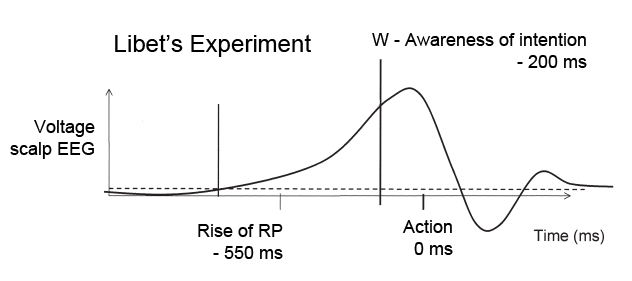
\includegraphics[width=0.9\textwidth,natwidth=632,natheight=281]{./Figures/LibetExperiment.png}
\caption{LibetExperiment}
\end{figure}

[ ref ][ ref ]
With the fact that there is measurable data from an EEG to discern that movements are coming it would be a minimal feature to look for in the data from the EPOC.

\subsection{Put this some where}
Tried both direction based and raw data(say it wasn't just the second before the event) for the Naive Bayes, Bayes net and Multilayered perceptron in weka.

\section{Artificial neural nets:}
- [introduction to Neural networks in c\#] -
number of hidden layers
layers
none - only capable of representing linear separable functions of decisions
one - can approximate any function that contains a continuous mapping from one finite space to another
two - can represent an arbitrary decision boundary to a arbitrary accuracy with rational activation functions and can approximate any smooth mapping to any accuracy
one hidden layer is practical for most any function
there is no theoretical reason to go to more than 2 layers 
the number of neurons in the hidden layer
underfitting - too few neurons in hidden layer
not good for a complicated data set
To many may result in overfitting
limited information is not enough to train all the hidden layers neurons
sufficient info - to many neurons - too much training time.
Rules of thumb
number of neurons between the number of output and input neuron number
hidden neurons 2/3 size of input plus number of output
number of hidden neurons less than twice the size of the input layer
You will have to ultimately try various numbers of Hidden neurons - kurzweil says evolutionary algorithms.
this can also give you specialized neural nets that may be better for some but not other applications.

IMAGE OF CORTICAL COLUMN

\section {Real Neural Networks}

Information processing in animals is done with networks of neurons. In vertebrates its done in large networks of neurons called brains. Humans have an advanced brain capable of simulating the environment and planning for the long term future. 

What is the brain
    The brain is a approximately 1.5kg mass of information processing and support cells. The brain is composed of many different structures. Cerebellum is a largely repetitive structure primarily used for motor learning and fine control located at the base of the brain. Brainstem consists of a few sub regions. At the top of the spinal cord is the Medulla oblongata which contains many of the automatic functions to maintain homeostasis such as heart rate, and breathing . Above the medulla is the Pons which has white matter tracts to move information to and from the body. The pons also has some regulatory functions such as helping control the muscles of the face, eyes and throat, equilibrium, hearing and taste and facial sensations. The last region in the brain stem is midbrain � vision, hearing, motor control, sleep/wake, arousal (alertness), and temperature regulation.[2]�. 

The Thalamus is a region of the brain above the brainstem.
Limbic .
Cerebral cortex .
The Cerebral cortex is divided into four main lobes. The occipital, parietal, temporal and frontal, 
White matter .
Grey matter .

\begin{figure}[h!]
\centering
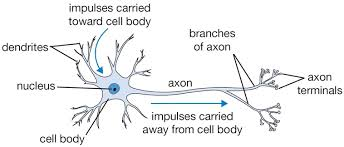
\includegraphics[width=1.4\textwidth,natwidth=535,natheight=308]{./Figures/Neuron.jpg}
\caption{Basic neuron}
\end{figure}
IMAGE OF NEURON

The brain is made up of two types of cells Glia and Neurons are the main cells of the brain. Neurons are the main information processing units of the brain, with glia being an important partner cell to neurons. As they help to maintain the environment for neurons and help regulate synaptic connections. Neurons have some specializations that allow them to process information and pass the new information to any neurons that are connected to them. The specializations are the Axon and Dendrites. Axons are extensions from the Soma starting at the axon hillock.There primary purpose is to carry an action potential to the synaptic boutons. Action potentials will be discussed in more detail below. The axons can be myelinated or not by special glia. If they are myelinated they have a better conduction speed. This is due to the ability of the myelin to allow the voltage to be transmitted via saltatory conduction. The action potential is thus conducted past the section of the axon that is myelinated and to a section of the axon that is not myelinated. This unmyelinated section is called a node of Ranvier. At nodes of Ranvier the action potential is regenerated via the ion channels present in the cell membrane. If there are the axons are entirely non myelinated then the action potential is entirely transmitted with ion channels. 
Synapses occur between two neurons and are the location where information is passed from one neurons axon to its neighbors Dendrites. The synapses work either with a chemical or electrical connection[gap junction]. Chemical connections being the most common in vertebrate brains[ ?REF? ]. Chemical synapses work by the following mechanism. When the action potential reaches the location of a synapse it triggers neurotransmitter release. the voltage change from the action potential in the membrane opens up the local Ca+ ion channels. As the Ca+ ions build up in the synaptic bouton the Ca+ binds to the two binding sites on synaptotagmin.  vesicle(VAMP vSNARE), target membrane(syntaxin, snap25, tSNARE) [ snare complex ]
[ ref ] [ molecular mechanisms of neurotransmitter release ]

Dendrites are 
     the postsynaptic terminal 
    dendrites work to sum the incoming information of the connected synapses.
    
how spikes are generated, 
    Action potentials
        voltage gated ion channels
how signals are transmitted 
    chemical 
    gap 
networks in the brain 
    columns
top down processing 
bottom up processing


Human brain < i guess this should be in a discussion about ann and how they compair with the human brain.>
~100 Billion neurons
~100 Trillion synapses
~300 Million minicolumns.
~80-120 Neurons in a minicolumn
~1000-10,000 Inputs/cell
~700 New neurons every day [ ?ref? ]

\section {Liquid State Machine}

separation property a measure of the euclidean distance of the states of the network with different samples. 
%http://www.phil.uu.nl/preprints/ckiscripties/SCRIPTIES/067_matser.pdf
also good at approximation


4. Make it exciting, make it current, make it important - why do I want to keep
reading?
Why is it current?
Brain Computer interfaces are coming of age. The work of Miguel Nicolelis.
One of the issues with brain computer interfaces for humans though is that they would require an invasive procedures. Some could be optogenetic (I think this is the most promising) or micro electrode array. The procedures for these technologies have potentially adverse health effects. These health effects range from inflammation around areas where surgery was performed to death. anytime you have major surgery you have the potential for death. optogenetic interfaces in adult animals

Why is it new?
Its new because it uses a liquid state machine in the configuration of the mammalian auditory system.
the use of a fourier transform for the first part of the processing is ?unique. (<todo> has this been done before</todo>). this should allow for more modularity in the structure of the lsm. it is also closer to how natural systems have come to good solutions for the processing of data that is frequency based and spatial temporal.



5. Should you list here the solutions from other researchers? I think not, list
instead the different facets of the problems that other researchers have attacked.
:facets - 



6. A taxonomy can be extremely useful to place your problem and its particular
special features within the perfect context of the overall area, as you need to
make sure that the reader understands perfectly what you are trying to solve.








\setlength{\unitlength}{\savedunitlength}

  \startchapter{The New Approach and Solution}
\label{chapter:newsol}

This is where you go all out and tell us all about your new discovery and research related to the problem in the previous chapter. No arrogant sweeping statements which cannot be fully justified, but no false modesty either. You must impress your reader that you have accomplished something.

Simply summarized, this chapter should be comprised of at least two main sections, each with appropriate subsections. The first section should describe:
\begin{itemize}
\item {what the new approach is;}
\item {what is really totally new;}
\item {what is incrementally new;}
\item {what you built upon.}
\end{itemize}

The second part should describe fully how the new approach works, both with the overall theoretical exposition (e.g. an algorithm) and with as many examples as necessary for clarity. Remember that if the reader does not understand fully, you will get a lot of questions and doubts. Good examples, good figures, good diagrams with super clear tutorial explanations can be a joy to read and make even a small contribution appear to be more impressive. Are you afraid that if you are too tutorial your work will not seem as deep and difficult? Only shallow people will make such a superficial evaluation, have trust instead in the wisdom of your supervisory committee.

Use at least one good example throughout, and even better if this is one of the examples you used in Chapter 2 to describe the original problem.

By the way, this would be the first chapter I would write. This is what I know best right now, as I just finished working on it. It is clear to me and on the tip of my fingers. Start with your strengths! The second chapter I would write is the next one about the experiments, followed closely by chapter 2 describing the problem. It may not seem intuitive to you, but it works and it is the most productive way I ever found to finish a document.


\input chapters/3/sec_latexhelp

  \startchapter{Experiments}
\label{chapter:Exp}

Assuming you have some experimental results to support your claims this is where all the data is reported. There are a few issues you should consider before dumping a lot of stuff here, or it will lose its effectiveness.

First of all you must describe precisely the experimental setup and the benchmarks you used. In any scientific discipline an experimental result is only good if it is reproducible. To be reproducible then somebody else must have sufficient details of the setup to be able to obtain the same data. Thus the first section in this chapter is a super precise history of the decisions made towards experimentation, including mentions of the paths which became infeasible. The setup must be valid and thus your description of it must prove that it is indeed sound. At times, terrifying times, when writing this section, both supervisor and student realize belatedly that something is missing and more work needs to be done!

The second portion of this chapter is dedicated the the actual results. At least two issues arise here:
\begin{enumerate}
\item {Should all the data be reported here or should some be placed in the Appendix?}
\item {Should this be an exposition of the raw facts and data or should it include its analysis and evaluation?}
\end{enumerate}

There are no definite answers here, but I follow a few rules.

\textit{Should all the data be reported here or should some be placed in the Appendix?}
    \begin{itemize}
    \item{If there is a large number of tables of data, it might be better to present here only a handful of the most significant ("best") results, leaving all the rest of the data in the Appendix with proper linkages, as it would make the chapter so much more easily readable (not to mention limiting the struggle with a word processor for the proper placement of tables and text).}
    \item{Use an example throughout, call it a "case study" to make it sound better, so that all the data and results are somehow linked in their logic, and even better if this is one of the examples you used in Chapter 2 to describe the original problem.}
    \item{Highlight in some manner the important new data, for example the column of your execution speed where all the numbers are much smaller. Make the results highly easy to read!}
    \item{It is normally expected that data should be presented only in one form and not duplicated, that is, you are not supposed to include both a table of raw numbers and also its graphical representation from some wonderful Excel wizard. I tend to disagree. I would not wish to see every results repeated in this manner, but some crucial ones need to be seen in different manners, even with the same information content, in order to show their impact. One good trick is to place the more boring tables in the Appendix and use wonderful graphs in this chapter.}
    \item{This is the one chapter where I would splurge and use colour printing where necessary, as it makes an \textit{enourmous} difference.}
    \end{itemize}

\textit{Should this be an exposition of the raw facts and data or should it include its analysis and evaluation?}
     \begin{itemize}
    \item{Is the evaluation of the data really obvious? For example you have 10 tables to show that your chemical process is faster in development and gives purer material - you may simply need to highlight one column in each table and state the obvious.}
    \item{Most results are not that obvious even if they appear so. Moreover this is where you are comparing your \textit{new} results to data from other people. I usually describe other people's work at this point and make comparisons. That is why I prefer to talk about the analysis and evaluation of the results in a separate chapter.}
    \item{There is absolutely no clear structure here which is best.}
    \end{itemize}

  \startchapter{Evaluation, Analysis and Comparisons}
\label{chapter:eval}

For a Master's research this chapter represents the critical part where \textbf{you} are truly evaluated to determine whether you should be given your degree. Even more so for a PhD. Consider carefully what the University calendar states regarding the expectations for a master's thesis, paraphrased here.

\begin{enumerate}
\item {\textit{A Master�s thesis is an original lengthy essay.} The main implication here is that the essay is original, that is, it is completely newly written by you and does not contain any writings from others unless precisely quoted. Any paraphrased items must be cited.}
\item {\textit{It must demonstrate that:}
    \begin{itemize}
    \item {students understand research methods;}
    \item {students are capable to employ research methods;}
    \item {students demonstrate command of the subject.}
    \end{itemize}}
\item {\textit{The work may be based on:}
    \begin{itemize}
    \item {original data;}
    \item {original exercise from scholarly literature;}
    \item {data by others.}
    \end{itemize}}
\item {\textit{The work must show that:}
    \begin{itemize}
    \item {appropriate research methods have been used;}
    \item {appropriate methods of critical analysis supplied.}
    \end{itemize}}
\item {\textit{The work must contain:}
    \begin{itemize}
    \item {evidence of some new contribution;}
    \item {evidence of a new perspective on existing knowledge.}
    \end{itemize}}
\end{enumerate}

Only the last point uses the attribute \textit{new} and it refers almost entirely to giving a new perspective and analysis, even if based on data from others. This truly implies that this current chapter on evaluation and analysis of results is the most important and must be written with care. You are demonstrating here that, even if given data and methods from others, your skills of critical judgment and analysis are now at the level that you can give professional evaluations.

Things are slightly different for a PhD. According to the Graduate Calendar: \\ 
\textit{a doctoral dissertation must embody original work and constitute a significant contribution to knowledge in the candidate's field of study. It should contain evidence of broad knowledge of the relevant literature, and should demonstrate a critical understanding of the works of scholars closely related to the subject of the dissertation. Material embodied in the dissertation should, in the opinion of scholars in the field, merit publication.}

\textit{The general form and style of dissertations may differ from department to department, but all dissertations shall be presented in a form which constitutes an integrated submission. The dissertation may include materials already published by the candidate, whether alone or in conjunction with others. Previously published materials must be integrated into the dissertation while at the same time distinguishing the student's own work from the work of other researchers. At the final oral examination, the doctoral candidate is responsible for the entire content of the dissertation. This includes those portions of co-authored papers which comprise part of the dissertation.}

The second paragraph makes it clear that one must emphasize what is new and different from others, without arrogance, yet without being too subtle either. The first paragraph implies that for a PhD it is required that one approached an important open problem and gave a new solution altogether, making chapters 3, 4, 5 all part of the body of research being evaluated. In fact at times even the problem may be entirely new, thus including chapter 2 in the examination. This is in contrast to a Master's degree where the minimum requirement is for chapter 5 to be original.




  \startchapter{Conclusions}
\label{concl}

My first rule for this chapter is to avoid finishing it with a section talking about future work. It may seem logical, yet it also appears to give a list of all items which remain undone! It is not the best way psychologically.

This chapter should contain a mirror of the introduction, where a summary of the \textit{extraordinary} new results and their wonderful attributes should be stated first, followed by an executive summary of how this new solution was arrived at. Consider the practical fact that this chapter will be read quickly at the beginning of a review (thus it needs to provide a strong impact) and then again in depth at the very end, perhaps a few days after the details of the previous 3 chapters have been somehow forgotten. Reinforcement of the positive is the key strategy here, without of course blowing hot air.

One other consideration is that some people like to join the chapter containing the analysis with the only with conclusions. This can indeed work very well in certain topics.

Finally, the conclusions do not appear only in this chapter. This sample mini thesis lacks a feature which I regard as absolutely necessary, namely a short paragraph at the end of each chapter giving a brief summary of what was presented together with a one sentence preview as to what might expect the connection to be with the next chapter(s). You are writing a story, the \textit{story of your wonderful research work}. A story needs a line connecting all its parts and you are responsible for these linkages.

  \appendix
  \startappendix{Additional Information}
\label{chapter:appendix}

This is a good place to put tables, lots of results, perhaps all the data compiled in the experiments. By avoiding putting all the results inside the chapters themselves, the whole thing may become much more readable and the various tables can be linked to appropriately.

The main purpose of an Appendix however should be to take care of the future readers and researchers. This implies listing all the housekeeping facts needed to continue the research. For example: where is the raw data stored? where is the software used? which version of which operating system or library or experimental equipment was used and where can it be accessed again?

Ask yourself: if you were given this thesis to read with the goal that you will be expanding the research presented here, what would you like to have as housekeeping information and what do you need? Be kind to the future graduate students and to your supervisor who will be the one stuck in the middle trying to find where all the stuff was left!



% The style of bibliography exemplified here is the "plain",
% normally used in science theses. This is shown
% by the entry {plain} below. Substitute the
% appropriate bibliography style. See also the
% PDF file "InformationOnBibliographyStyles" in this
% directory for more choices.

% The Bibliography file is a BibTex file named
% UVicThesis.bib and called below

  \TOCadd{Bibliography}
  \bibliographystyle{plain}
  \bibliography{UvicThesis}

\end{document}
